\documentclass[11pt]{article}
\usepackage[margin=0.8in]{geometry}
\usepackage{amsmath, amssymb}
\usepackage{booktabs}
\usepackage{array}
\usepackage{enumitem}
\usepackage{fancyhdr}
\usepackage{parskip}
\usepackage{bm}
\usepackage{tikz}
\usetikzlibrary{shapes,arrows,positioning}

% Header and Footer
\pagestyle{fancy}
\setlength{\headheight}{13.6pt}
\fancyhf{}
\fancyhead[C]{\textbf{Chapter 2: Probability Summary Notes}}
\fancyfoot[C]{CEE 305 - Spring 2026}
\renewcommand{\headrulewidth}{1pt}
\renewcommand{\footrulewidth}{0.5pt}

\begin{document}

% ==========================================
\section*{Introduction to Probability}
% ==========================================
Probability theory provides a mathematical framework for quantifying uncertainty. This chapter covers basic definitions, set operations, counting methods, conditional probability, random variables, and joint distributions.

% ==========================================
\section*{Section 2.1: Basic Ideas and Definitions}
% ==========================================
\subsection*{Fundamental Definitions}
\begin{itemize}[nosep]
    \item \textbf{Experiment:} A process that results in an outcome that cannot be predicted in advance with certainty.
    \item \textbf{Sample Space (S):} The set of all possible outcomes of an experiment.
    \item \textbf{Event:} A subset of a sample space. An event occurs if the outcome of the experiment is one of the outcomes in the event.
\end{itemize}

\subsection*{Examples of Sample Spaces}
\begin{itemize}[nosep]
    \item Rolling a die: \(S = \{1, 2, 3, 4, 5, 6\}\)
    \item Tossing a coin: \(S = \{\text{heads, tails}\}\)
    \item Weighing a cereal box: \(S = (0, \infty)\) or more realistically \((12, 20)\) for a 16 oz. box
\end{itemize}

\subsection*{Types of Events}
\begin{itemize}[nosep]
    \item \textbf{Simple event:} An event that cannot be decomposed further
    \item \textbf{Mutually exclusive events:} Events that have no outcomes in common; when one occurs, the other cannot
\end{itemize}

\subsection*{Set Operations on Events}

\subsubsection*{The Union Operator (\(\cup\))}
\textbf{Definition:} \(A \cup B = \{x : x \in A \text{ or } x \in B\}\) (outcomes in either A or B or both).

\begin{center}
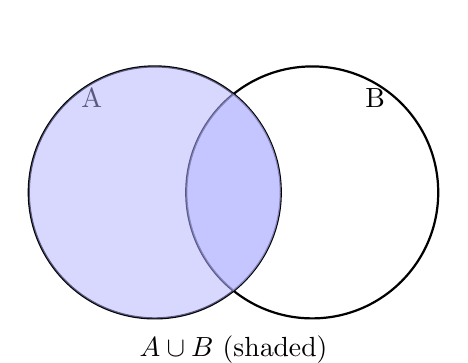
\begin{tikzpicture}[scale=0.8]
\draw[thick] (0,0) circle (2);
\draw[thick] (2.5,0) circle (2);
\node at (-1,1.5) {A};
\node at (3.5,1.5) {B};
\begin{scope}
\clip (0,0) circle (2);
\fill[blue!30, opacity=0.5] (2.5,0) circle (2);
\end{scope}
\fill[blue!30, opacity=0.5] (0,0) circle (2);
\node at (1.25,-2.5) {\(A \cup B\) (shaded)};
\end{tikzpicture}
\end{center}

\subsubsection*{The Intersection Operator (\(\cap\))}
\textbf{Definition:} \(A \cap B = \{x : x \in A \text{ and } x \in B\}\) (outcomes in both A and B).

\begin{center}
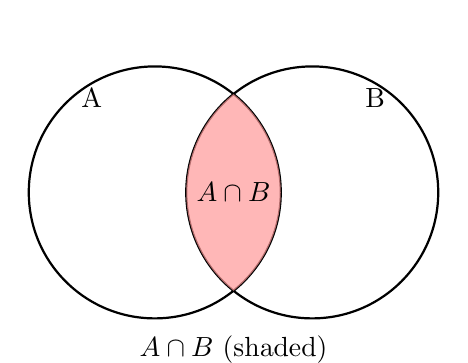
\begin{tikzpicture}[scale=0.8]
\draw[thick] (0,0) circle (2);
\draw[thick] (2.5,0) circle (2);
\node at (-1,1.5) {A};
\node at (3.5,1.5) {B};
\begin{scope}
\clip (0,0) circle (2);
\fill[red!40, opacity=0.7] (2.5,0) circle (2);
\end{scope}
\node at (1.25,0) {\(A \cap B\)};
\node at (1.25,-2.5) {\(A \cap B\) (shaded)};
\end{tikzpicture}
\end{center}

\subsubsection*{The Complement Operator (\(^c\))}
\textbf{Definition:} \(A^c = \{x \in S : x \notin A\}\) (all outcomes not in A).

\begin{center}
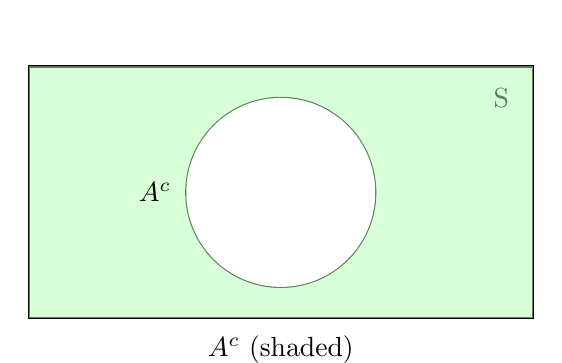
\begin{tikzpicture}[scale=0.8]
\draw[thick] (-3,-2) rectangle (5,2);
\node at (4.5,1.5) {S};
\draw[thick] (1,0) circle (1.5);
\node at (1,0.8) {A};
\fill[green!30, opacity=0.5] (-3,-2) rectangle (5,2);
\begin{scope}
\clip (1,0) circle (1.5);
\fill[white] (-3,-2) rectangle (5,2);
\end{scope}
\node at (-1,0) {\(A^c\)};
\node at (1,-2.5) {\(A^c\) (shaded)};
\end{tikzpicture}
\end{center}

\subsubsection*{Mutually Exclusive (Disjoint) Events}
\(A\) and \(B\) are mutually exclusive if \(A \cap B = \emptyset\).

\begin{center}
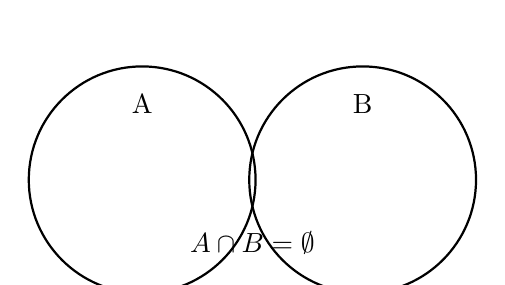
\begin{tikzpicture}[scale=0.8]
\draw[thick] (0,0) circle (1.8);
\draw[thick] (3.5,0) circle (1.8);
\node at (0,1.2) {A};
\node at (3.5,1.2) {B};
\node at (1.75,-1) {\(A \cap B = \emptyset\)};
\end{tikzpicture}
\end{center}

\subsubsection*{Key Relationships and Rules}
\begin{align*}
    \textbf{De Morgan's Laws:}&\quad (A \cup B)^c = A^c \cap B^c,\qquad (A \cap B)^c = A^c \cup B^c\\
    \textbf{Distributive Laws:}&\quad A \cap (B \cup C) = (A \cap B) \cup (A \cap C),\quad A \cup (B \cap C) = (A \cup B) \cap (A \cup C)\\
    \textbf{Complement Laws:}&\quad A \cup A^c = S,\quad A \cap A^c = \emptyset,\quad (A^c)^c = A
\end{align*}

\subsection*{Probability Axioms and Rules}
\begin{itemize}[nosep]
    \item \(0 \leq P(A) \leq 1\)
    \item \(P(S) = 1\)
    \item If \(A\) and \(B\) are mutually exclusive, \(P(A \cup B) = P(A) + P(B)\)
    \item \(P(A^c) = 1 - P(A)\)
    \item \(P(\emptyset) = 0\)
\end{itemize}

\textbf{General Addition Rule:} \(P(A \cup B) = P(A) + P(B) - P(A \cap B)\)

\begin{center}
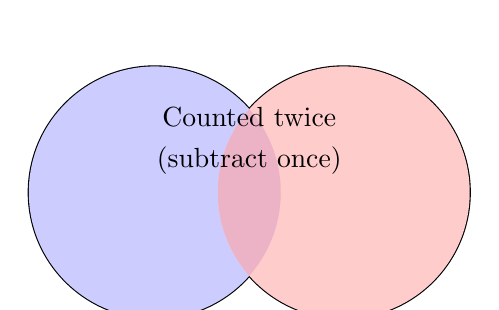
\begin{tikzpicture}[scale=0.8]
\draw[thick] (0,0) circle (2);
\draw[thick] (3,0) circle (2);
\node at (-1,1.5) {A};
\node at (4,1.5) {B};
\fill[blue!20] (0,0) circle (2);
\fill[red!20] (3,0) circle (2);
\begin{scope}
\clip (0,0) circle (2);
\fill[purple!30] (3,0) circle (2);
\end{scope}
\node at (1.5,1.2) {Counted twice};
\node at (1.5,0.5) {(subtract once)};
\end{tikzpicture}
\end{center}

\textbf{Equally Likely Outcomes:} If \(S\) has \(N\) equally likely outcomes and \(A\) contains \(k\) outcomes, \(P(A) = k/N\).

% ==========================================
\section*{Section 2.2: Counting Methods}
% ==========================================
\textbf{Fundamental Principle of Counting:} \(n_1 \times n_2 \times \cdots \times n_k\)

\textbf{Permutations (order matters):}
\begin{itemize}[nosep]
    \item Permutations of \(n\) distinct objects: \(n!\)
    \item Permutations of \(k\) objects chosen from \(n\): \(P^n_k = \frac{n!}{(n-k)!}\)
\end{itemize}

\textbf{Combinations (order does not matter):}
\[
\binom{n}{k} = \frac{n!}{k!(n-k)!}
\]

\textbf{Multinomial coefficient:} \(\frac{n!}{k_1!k_2!\cdots k_r!}\) where \(k_1+\cdots+k_r=n\).

% ==========================================
\section*{Section 2.3: Conditional Probability and Independence}
% ==========================================
\textbf{Conditional Probability:} \(P(A|B) = \frac{P(A \cap B)}{P(B)},\quad P(B)>0\)

\begin{center}
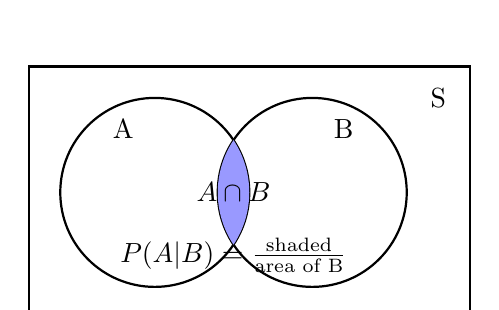
\begin{tikzpicture}[scale=0.8]
\draw[thick] (-2,-1) rectangle (5,3);
\node at (4.5,2.5) {S};
\draw[thick] (0,1) circle (1.5);
\draw[thick] (2.5,1) circle (1.5);
\node at (-0.5,2) {A};
\node at (3,2) {B};
\begin{scope}
\clip (0,1) circle (1.5);
\fill[blue!40] (2.5,1) circle (1.5);
\end{scope}
\node at (1.25,1) {\(A \cap B\)};
\node at (1.25,0) {\(P(A|B) = \frac{\text{shaded}}{\text{area of B}}\)};
\end{tikzpicture}
\end{center}

\textbf{Multiplication Rule:} \(P(A \cap B) = P(A|B)P(B) = P(B|A)P(A)\)

\textbf{Independence:} \(A\) and \(B\) independent if \(P(A \cap B) = P(A)P(B)\) (equivalently \(P(A|B)=P(A)\) or \(P(B|A)=P(B)\)).

\textbf{Law of Total Probability:} If \(A_1,\dots,A_n\) partition \(S\), then \(P(B) = \sum_{i=1}^n P(B|A_i)P(A_i)\).

\textbf{Bayes' Theorem:}
\[
P(A_k|B) = \frac{P(B|A_k)P(A_k)}{\sum_{i=1}^n P(B|A_i)P(A_i)}
\]

% ==========================================
\section*{Section 2.4: Random Variables}
% ==========================================
\textbf{Random Variable:} A numerical value assigned to each outcome of an experiment.

\subsection*{Discrete Random Variables}
Probability mass function (PMF): \(p(x)=P(X=x)\) with \(0\le p(x)\le1\) and \(\sum p(x)=1\).

Cumulative distribution function (CDF): \(F(x)=P(X\le x)=\sum_{t\le x}p(t)\).

\textbf{Mean:} \(\mu_X = E(X) = \sum x\,p(x)\)

\textbf{Variance:} \(\sigma_X^2 = V(X) = \sum (x-\mu_X)^2 p(x) = \sum x^2 p(x) - \mu_X^2\)

\textbf{Standard deviation:} \(\sigma_X = \sqrt{\sigma_X^2}\)

\subsection*{Continuous Random Variables}
Probability density function (PDF): \(f(x)\) with \(\int_{-\infty}^{\infty} f(x)dx=1\), \(P(a\le X\le b)=\int_a^b f(x)dx\), and \(P(X=a)=0\).

CDF: \(F(x) = \int_{-\infty}^x f(t)dt\)

\textbf{Mean:} \(\mu_X = \int_{-\infty}^{\infty} x f(x)dx\)

\textbf{Variance:} \(\sigma_X^2 = \int (x-\mu_X)^2 f(x)dx = \int x^2 f(x)dx - \mu_X^2\)

\subsection*{Percentiles and Median}
\(p\)th percentile \(x_p\) satisfies \(F(x_p)=p/100\). Median = 50th percentile.

\subsection*{Chebyshev's Inequality}
For any \(k>0\): \(P(|X-\mu_X|\ge k\sigma_X) \le 1/k^2\). (Holds for any distribution.)

% ==========================================
\section*{Section 2.5: Linear Functions of Random Variables}
% ==========================================
\textbf{Single linear transformation:}
\[
\mu_{aX+b}=a\mu_X+b,\quad \sigma_{aX+b}^2=a^2\sigma_X^2,\quad \sigma_{aX+b}=|a|\sigma_X
\]

\textbf{Linear combination (mean):}
\[
\mu_{c_1X_1+\cdots+c_nX_n}=c_1\mu_{X_1}+\cdots+c_n\mu_{X_n}
\]

\textbf{Variance for independent variables:}
\[
\sigma_{c_1X_1+\cdots+c_nX_n}^2 = c_1^2\sigma_{X_1}^2+\cdots+c_n^2\sigma_{X_n}^2
\]
Special cases: \(\sigma_{X+Y}^2=\sigma_X^2+\sigma_Y^2\), \(\sigma_{X-Y}^2=\sigma_X^2+\sigma_Y^2\).

\textbf{Sample mean:} For i.i.d. sample \(X_1,\dots,X_n\) with mean \(\mu\) and variance \(\sigma^2\):
\[
\mu_{\bar{X}}=\mu,\quad \sigma_{\bar{X}}^2=\frac{\sigma^2}{n},\quad \sigma_{\bar{X}}=\frac{\sigma}{\sqrt{n}}
\]

% ==========================================
\section*{Section 2.6: Jointly Distributed Random Variables}
% ==========================================
\subsection*{Joint PMF (discrete)}
\(p(x,y)=P(X=x,Y=y)\), \(\sum_x\sum_y p(x,y)=1\)

Marginal PMFs: \(p_X(x)=\sum_y p(x,y)\), \(p_Y(y)=\sum_x p(x,y)\)

\subsection*{Joint PDF (continuous)}
\(f(x,y)\) with \(\int_{-\infty}^{\infty}\int_{-\infty}^{\infty} f(x,y)\,dy\,dx=1\)
\[
P(a\le X\le b, c\le Y\le d)=\int_a^b\int_c^d f(x,y)\,dy\,dx
\]
Marginal PDFs: \(f_X(x)=\int_{-\infty}^{\infty} f(x,y)\,dy\), \(f_Y(y)=\int_{-\infty}^{\infty} f(x,y)\,dx\)

\subsection*{Conditional Distributions}
Discrete: \(p_{Y|X}(y|x)=\frac{p(x,y)}{p_X(x)}\); Continuous: \(f_{Y|X}(y|x)=\frac{f(x,y)}{f_X(x)}\)

\subsection*{Independence}
\(X\) and \(Y\) independent iff \(p(x,y)=p_X(x)p_Y(y)\) (discrete) or \(f(x,y)=f_X(x)f_Y(y)\) (continuous). Then \(E(XY)=E(X)E(Y)\).

\subsection*{Covariance and Correlation}
\[
\operatorname{Cov}(X,Y)=E[(X-\mu_X)(Y-\mu_Y)]=E(XY)-\mu_X\mu_Y
\]
\[
\rho_{X,Y}=\frac{\operatorname{Cov}(X,Y)}{\sigma_X\sigma_Y},\quad -1\le\rho\le1
\]
If independent, \(\operatorname{Cov}=0\) (but not vice versa).

\subsection*{Variance of Linear Combinations (General)}
\[
\operatorname{Var}\left(\sum c_i X_i\right)=\sum c_i^2\sigma_{X_i}^2+2\sum_{i<j}c_ic_j\operatorname{Cov}(X_i,X_j)
\]

% ==========================================
\section*{Summary Tables}
% ==========================================
\subsection*{Set Operations}
\begin{center}
\begin{tabular}{l l l}
\toprule
\textbf{Operation} & \textbf{Notation} & \textbf{Meaning} \\
\midrule
Union & \(A \cup B\) & A or B (or both) \\
Intersection & \(A \cap B\) & A and B \\
Complement & \(A^c\) & Not A \\
Difference & \(A \setminus B\) & A but not B \\
Empty set & \(\emptyset\) & No outcomes \\
Sample space & \(S\) & All outcomes \\
\bottomrule
\end{tabular}
\end{center}

\subsection*{Probability Rules}
\begin{center}
\begin{tabular}{l l}
\toprule
\textbf{Rule} & \textbf{Formula} \\
\midrule
Complement & \(P(A^c)=1-P(A)\) \\
Addition (mutually exclusive) & \(P(A\cup B)=P(A)+P(B)\) \\
Addition (general) & \(P(A\cup B)=P(A)+P(B)-P(A\cap B)\) \\
Multiplication (general) & \(P(A\cap B)=P(A|B)P(B)\) \\
Multiplication (independent) & \(P(A\cap B)=P(A)P(B)\) \\
Conditional probability & \(P(A|B)=\frac{P(A\cap B)}{P(B)}\) \\
Law of total probability & \(P(B)=\sum_i P(B|A_i)P(A_i)\) \\
Bayes' theorem & \(P(A_k|B)=\frac{P(B|A_k)P(A_k)}{\sum_i P(B|A_i)P(A_i)}\) \\
\bottomrule
\end{tabular}
\end{center}

\subsection*{Counting Methods}
\begin{center}
\begin{tabular}{l l}
\toprule
\textbf{Method} & \textbf{Formula} \\
\midrule
Fundamental counting principle & \(n_1\times n_2\times\cdots\times n_k\) \\
Permutations of \(n\) & \(n!\) \\
Permutations (\(k\) from \(n\)) & \(\frac{n!}{(n-k)!}\) \\
Combinations (\(k\) from \(n\)) & \(\binom{n}{k}=\frac{n!}{k!(n-k)!}\) \\
Multinomial coefficient & \(\frac{n!}{k_1!k_2!\cdots k_r!}\) \\
\bottomrule
\end{tabular}
\end{center}

\subsection*{Random Variable Properties}
\begin{center}
\begin{tabular}{l l}
\toprule
\textbf{Quantity} & \textbf{Formula} \\
\midrule
Mean (discrete) & \(\mu_X=\sum x\,p(x)\) \\
Mean (continuous) & \(\mu_X=\int x f(x)dx\) \\
Variance (discrete) & \(\sigma_X^2=\sum (x-\mu_X)^2 p(x)=\sum x^2 p(x)-\mu_X^2\) \\
Variance (continuous) & \(\sigma_X^2=\int (x-\mu_X)^2 f(x)dx=\int x^2 f(x)dx-\mu_X^2\) \\
Linear transformation & \(\mu_{aX+b}=a\mu_X+b,\; \sigma_{aX+b}=|a|\sigma_X\) \\
Sum of independent & \(\mu_{X+Y}=\mu_X+\mu_Y,\; \sigma_{X+Y}^2=\sigma_X^2+\sigma_Y^2\) \\
Sample mean & \(\mu_{\bar{X}}=\mu,\; \sigma_{\bar{X}}=\sigma/\sqrt{n}\) \\
Covariance & \(\operatorname{Cov}(X,Y)=E(XY)-\mu_X\mu_Y\) \\
Correlation & \(\rho_{X,Y}=\frac{\operatorname{Cov}(X,Y)}{\sigma_X\sigma_Y}\) \\
\bottomrule
\end{tabular}
\end{center}

% ==========================================
\section*{Definition of Symbols}
% ==========================================
{\small
\begin{center}
\begin{tabular}{l l}
\toprule
\textbf{Symbol} & \textbf{Definition} \\
\midrule
\(S\) & Sample space (set of all possible outcomes) \\
\(A, B, C\) & Events (subsets of \(S\)) \\
\(\emptyset\) & Empty set (impossible event) \\
\(A^c\) & Complement of \(A\) (not \(A\)) \\
\(A \cup B\) & Union of \(A\) and \(B\) (\(A\) or \(B\)) \\
\(A \cap B\) & Intersection of \(A\) and \(B\) (\(A\) and \(B\)) \\
\(P(A)\) & Probability of event \(A\) \\
\(P(A|B)\) & Conditional probability of \(A\) given \(B\) \\
\(n!\) & \(n\) factorial: \(n\times(n-1)\times\cdots\times1\) \\
\(\binom{n}{k}\) & Binomial coefficient: number of combinations of \(k\) from \(n\) \\
\(X, Y\) & Random variables \\
\(p(x)\) & Probability mass function (discrete) \\
\(f(x)\) & Probability density function (continuous) \\
\(F(x)\) & Cumulative distribution function \\
\(\mu_X\) or \(E(X)\) & Mean (expected value) of \(X\) \\
\(\sigma_X^2\) or \(V(X)\) & Variance of \(X\) \\
\(\sigma_X\) & Standard deviation of \(X\) \\
\(\bar{X}\) & Sample mean \\
\(\operatorname{Cov}(X,Y)\) & Covariance between \(X\) and \(Y\) \\
\(\rho_{X,Y}\) & Correlation coefficient between \(X\) and \(Y\) \\
\(p_{Y|X}(y|x)\) & Conditional PMF of \(Y\) given \(X=x\) \\
\(f_{Y|X}(y|x)\) & Conditional PDF of \(Y\) given \(X=x\) \\
\(a, b, c_i\) & Constants \\
\bottomrule
\end{tabular}
\end{center}
}

% ==========================================
\section*{Key Terminology}
% ==========================================
\begin{itemize}[nosep]
    \item \textbf{Experiment:} A process with uncertain outcomes.
    \item \textbf{Sample Space:} Set of all possible outcomes.
    \item \textbf{Event:} A subset of the sample space.
    \item \textbf{Mutually Exclusive:} Events that cannot occur simultaneously.
    \item \textbf{Conditional Probability:} Probability of an event given another has occurred.
    \item \textbf{Independence:} Occurrence of one event does not affect the probability of the other.
    \item \textbf{Random Variable:} A numerical function of outcomes.
    \item \textbf{PMF:} Probability mass function for discrete random variables.
    \item \textbf{PDF:} Probability density function for continuous random variables.
    \item \textbf{CDF:} Cumulative distribution function.
    \item \textbf{Expected Value:} Long-run average of a random variable.
    \item \textbf{Variance:} Measure of spread around the mean.
    \item \textbf{Covariance:} Measure of linear association between two variables.
    \item \textbf{Correlation:} Standardized covariance, ranging from \(-1\) to \(1\).
\end{itemize}

% ==========================================
\section*{Important Notes}
% ==========================================
\begin{itemize}[nosep]
    \item Probability is always between 0 and 1 inclusive.
    \item The complement rule is often the easiest way to compute \(P(A^c)\).
    \item For mutually exclusive events, the addition rule simplifies to \(P(A\cup B)=P(A)+P(B)\).
    \item Independence is a strong assumption; do not assume it without justification.
    \item Bayes' theorem is fundamental for updating beliefs with new data.
    \item The variance of the sample mean decreases as \(1/n\); more data reduces uncertainty.
    \item Covariance zero does NOT imply independence; there could be a nonlinear relationship.
    \item Chebyshev's inequality provides a worst-case bound, but the empirical rule (68–95–99.7) applies only to normal distributions.
\end{itemize}

\end{document}